\documentclass{simple}

\title[De ce să fii normal]{De ce să fii normal: O critică a exceselor lumii moderne}
\author[Răzvan Deaconescu]{Răzvan Deaconescu \\
razvan.deaconescu@upb.ro}
\date{11 februarie 2023}

\begin{document}

\frame{\titlepage}

\begin{frame}{}
  \begin{figure}
    \centering
    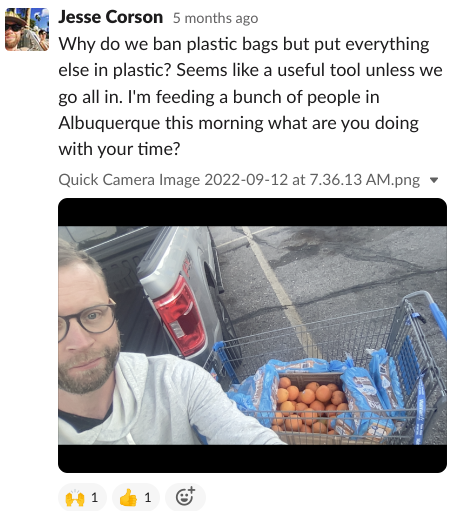
\includegraphics[width=0.7\textwidth]{img/plastic.png}
  \end{figure}
\end{frame}

\begin{frame}{Super-eroi}
  \begin{itemize}
    \pause \item Batman
    \pause \item Superman
    \pause \item Spiderman
    \pause \item Wolverine
  \end{itemize}
\end{frame}

\begin{frame}{Super-eroi (2)}
  \begin{itemize}
    \item ``The Boys'': Homelander, A-Train, The Deep, Black Noir, Queen Maeve
    \item ``Invincible'': Omni-Man, Rex Sloan
  \end{itemize}
\end{frame}

\begin{frame}{Who's Who?}
  \begin{itemize}
    \item Clifford E. Charlesworth, Gerald D. Griffin, Gene Kranz, Glynn Lunney, Milton Windler
    \item J.C.R. Licklider, Bob Taylor, Larry Roberts, Donald Davies, Paul Baran, Leonard Kleinrock
    \item George Brayton, Nicolaus Otto, Gottlieb Daimler, Wilhelm Maybach, Karl Benz, Rudolf Diesel
  \end{itemize}
\end{frame}

\begin{frame}{De ce nu normal / obișnuit?}
  \begin{itemize}
    \item viața e anti-entropică
    \item vrei să fii apreciat, iubit, văzut
    \item cel mai probabil lipsuri care caută compensare
  \end{itemize}
\end{frame}

\begin{frame}{De ce normal / obișnuit?}
  \begin{figure}
    \centering
    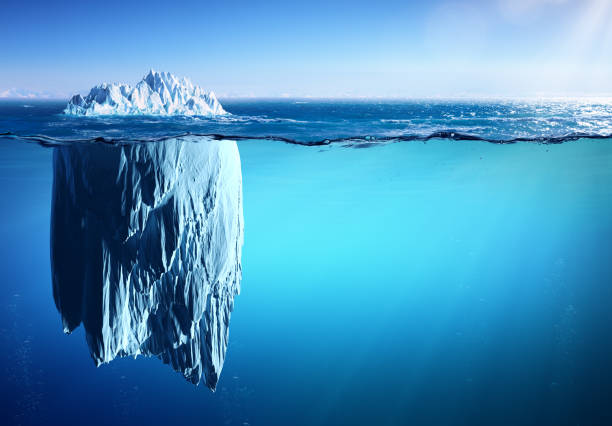
\includegraphics[width=0.7\textwidth]{img/iceberg.jpg}
  \end{figure}
\end{frame}

\begin{frame}{De ce normal / obișnuit? (2)}
  \begin{itemize}
    \pause \item cu puține lipsuri (deloc?)
    \pause \item cu puține insecurități (deloc?)
    \pause \item baza umană necesară pentru a construi (comunități, echipe, organizații, tehnologie)
  \end{itemize}
\end{frame}

\begin{frame}{(D)Efectele lipsei de normalitate}
  \begin{itemize}
    \pause
    \item status / virtue signaling
    \item centrul atenției
    \item (pasiv)agresivitate, defensivitate
    \item narcisism, ego-centrism, luat lucrurile personal
    \item insecurități, instabilitate
    \item neediness
    \item perspectivă negativă, justițiară: ,,lumea nu e OK''
  \end{itemize}
\end{frame}

\begin{frame}{Atributele normalității}
  \begin{itemize}
    \pause
    \item echilibru intern
    \item încredere în sine, împăcare cu sine
    \item acceptarea defectelor, acceptarea dubiilor
    \item self owned
    \item detașare, nu e nevoie să dovedești nimic
    \item ,,lumea e OK'', poate fi îmbunătățită
  \end{itemize}
\end{frame}

\begin{frame}{Recomandări}
  \begin{itemize}
    \pause \item meditație, analiză, timp petrecut cu sine
    \pause \item discuții profunde, chestionat, expus dubii, expus vulnerabilități
    \pause \item analiză critică, creștere, evoluție
    \pause \item acceptare, înțelegere (a ta, a celorlalți, a lumii)
    \pause \item fă lucruri, obține rezultate (mici, nu e cazul să fie extraordinare)
    \pause \item urmărește, rațional, statistici
    \pause \item be kind to others
    \pause \item nu te lua (prea) în serios
  \end{itemize}
\end{frame}

\begin{frame}{De final}
  \textit{
Vezi pe-un rege ce-mpânzește globu-n planuri pe un veac,\\
Când la ziua cea de mâine abia cuget-un sărac...\\
Deși trepte osebite le-au ieșit din urna sorții,\\
Deopotrivă-i stăpânește raza ta și geniul morții;\\
La același șir de patimi deopotrivă fiind robi,\\
Fie slabi, fie puternici, fie genii ori neghiobi!\\
  }
  \vspace{3mm}
  \hfill Mihai Eminescu, Scrisoarea I
\end{frame}

\end{document}
